
\section{Experimenting object affordances}

\ifverbose
The latest instantiation of the ``general principle'' we would like to
dwell upon is related to mirror neurons. It turns out that the causal
chain here is more compliceted. This requires a more complicated
structure to support it.
\fi

Poking moves us one step outwards on a causal chain away from the
robot and into the world, and gives a simple experimental procedure
for segmenting objects.  There are many possible elaborations of this
method, all of which lead to a vision system that is tuned to 
acquiring data about an object by seeing it manipulated by the robot.  

Segmentation alone is still unconvenient in many situation if not 
coupled with a mechanism to learn from experience. For example, it 
would be terribly unefficient to poke the object first and then try 
to grasp it. It would be much better if the robot could learn about
objects and [if it] had a way to identify a previously encountered object. 
A further difficulty, at least for a robot with a simple 
manipulator (e.g. as COG's flipper), is that ``affordances'' are scarce: 
most of the time the object simply move from one position
to another if we are willing to discount when it falls from the table.

However, for objects that roll there is a cue the robot can exploit
to understand their behavior. An object that rolls tends to do so even 
if it is not poked precisely. We selected a small set of objects to
experiment with: a cube, a toy car, an orange juice bottle, and a ball.
Affordances are not only a property of the mechanics of the object, but 
rather a combination of visual appearance, of the object's physical 
constituent, and of the ability of the actor. We selected a measure of
the principal axis of the object (easily obtained from the segmentation)
as visual component of the affordance. Table \ref{tab:affordances} shows the expected
behavior:

\begin{table*}[htbp]
\begin{center}
\begin{tabular}{|p{3.5cm}|p{3.5cm}|p{3.5cm}|}
\hline
{\it object} & {\it angle between principal axis and preferred direction of rolling} &  {\it behavior} \\ \hline\hline
{\bf cube} & n.a. & no principal axis, does not roll\\ \hline
{\bf car} & $0^\circ$ & rolls along the principal axis\\ \hline
{\bf bottle} &  $90^\circ$ & rolls at right angle\\ \hline
{\bf ball} &  n.a. & no principal axis, does roll\\ \hline
\end{tabular}
\caption{
\label{tab:affordances}
%
Behavior of a small set of objects when poked at random by the robot manipulator.
%
}
\end{center}
\end{table*}

A further elaboration is required to group the data belonging to the same
object as obtained from many poking acts in coherent clusters. As clustering 
mechanism we employed color histograms. After each poking action, a color histogram 
of the pixels of the segmented region is built and used as criterion 
to judge whether the object belongs to an existing group (i.e. if it
is mostly yellow, it is likely to be the toy car). This works well
for a limited set of objects but sophisticated methods are 
required for a more general case with many objects. 
The data structure that simulates the AIP-F5 affordance computation maintains all 
the instances of poking grouped by object, all the prototypes of the object segmented,
the direction of movement, and the action the robot applied in each particular case.

An alternative to the vision-based clustering procedure is to try to come 
to grips with the behavior of the objects after a single encounter, and use 
the behavior itself as clustering criterion. This is more difficult because 
of noise: e.g. there is still a non-zero probability that the object would 
not roll at all.

Figure \ref{fig:affordances} shows the results of the segmentation, clustering
and estimation of the affordance of the same set of four objects. The training set
consists of about 100 actions per object. The motor vocabulary of the robot
consists of four possible directions of poking. We labeled them for convenience
as: pull in, side tap, push away, and back slap, depending on the effect they
have on the object from the point of view of the robot. Actions were generated
at random during this training stage. During a poking action, the object is
tracked after the time of contact for 12 frames and the overall displacement is
estimated. 

\begin{figure}[tbh]
\begin{center}
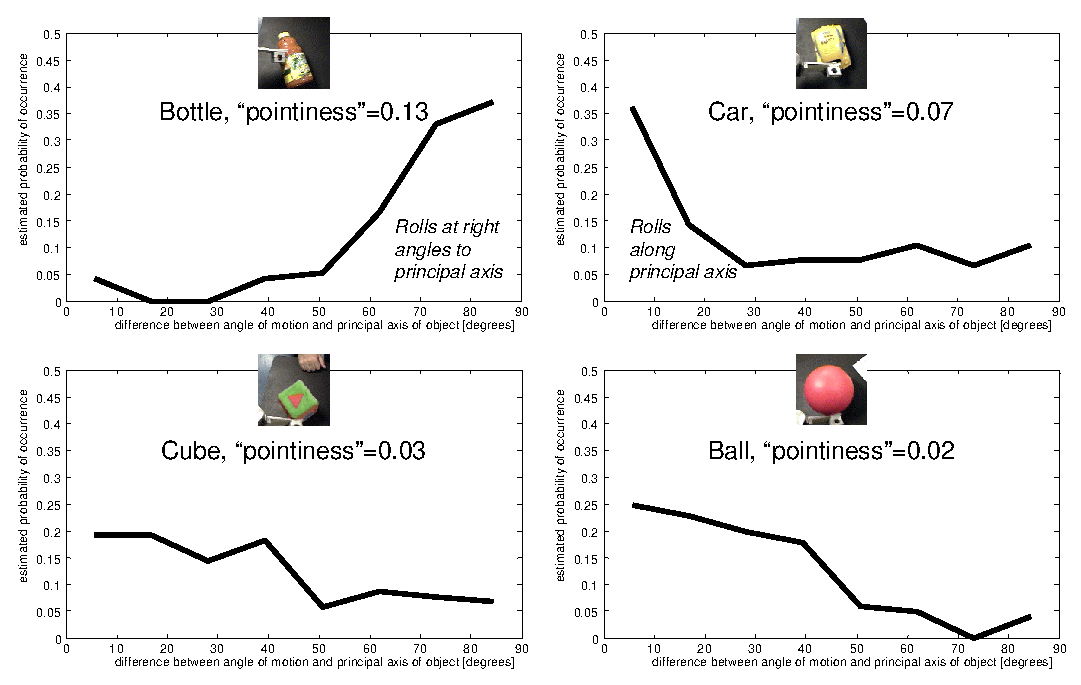
\includegraphics[width=\columnwidth]{affordances.eps}
\caption{ 
\label{fig:affordances}
%
Probability of observing a roll along a particular direction for the set
of four objects used in our experiments. Abscissae represent the difference
between the principal axis of the object and the observed direction of 
movement. Ordinates the estimated probability.
%
}
\end{center}
\end{figure}

Yet this description of the affordances does not have any usable quantity to 
take action once an object is observed. For this purpose a description of 
the geometry of poking is required: i.e. the description of the properties of 
objects (figure \ref{fig:affordances}) has to be connected to a description
of the behavior of the object. 
This information can be derived from the same training set we collected for learning
about rolling. Figure \ref{fig:actions} shows the histograms of the direction 
of movement of the object for
each possible action. For example, the back slap moves the object mostly upward
(about $-100^\circ$) and away from the robot. A similar consideration applies
to the other poking gestures. Figure \ref{fig:actions} was obtained from the data of
about 500 poking events.

The last step is to connect all these elements together. If a known object is
presented to COG, the object is recognized, localized, and
its orientation estimated. Recognition is based on the color histograms. The same
procedure used to form the clusters is employed here. Localization is simply implemented 
by histogram backprojection and a search across the image. The current orientation of the
object is then estimated by comparing the current image with all the prototypes 
contained in the cluster. 

To really exploit the understanding of the affordance we need to connect vision to 
behavior. The robot looks for the preferred rolling direction of the object
(see figure \ref{fig:affordances}) and adds it to its current orientation. 
The action whose effects are closer (on average) to the last sum is selected.

% TEST OF PERFORMANCE?

\begin{figure}[tb]
\begin{center}
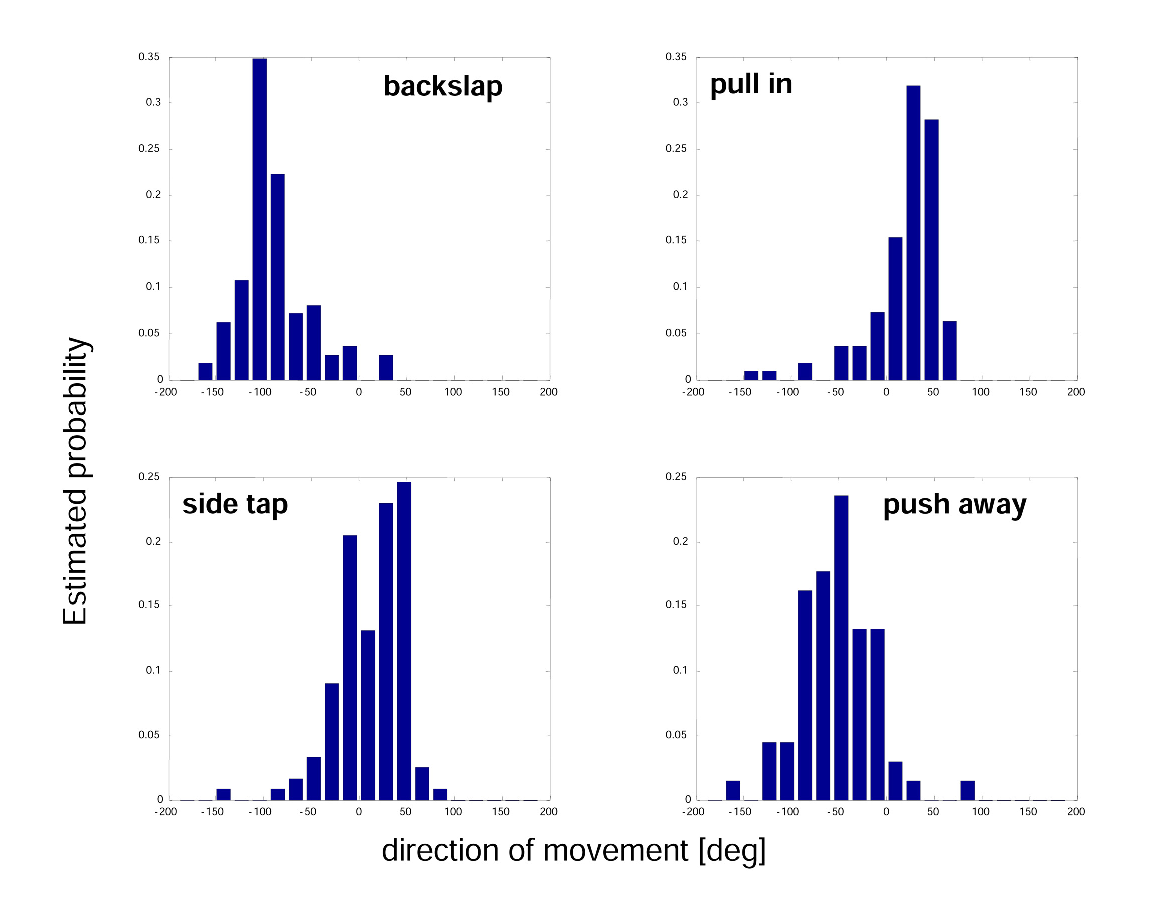
\includegraphics[width=8cm]{actions.eps}
\caption{ 
\label{fig:actions}
%
%
}
\end{center}
\end{figure}



\section{Developing mirror neurons?}


\begin{figure}[tb]
\begin{center}
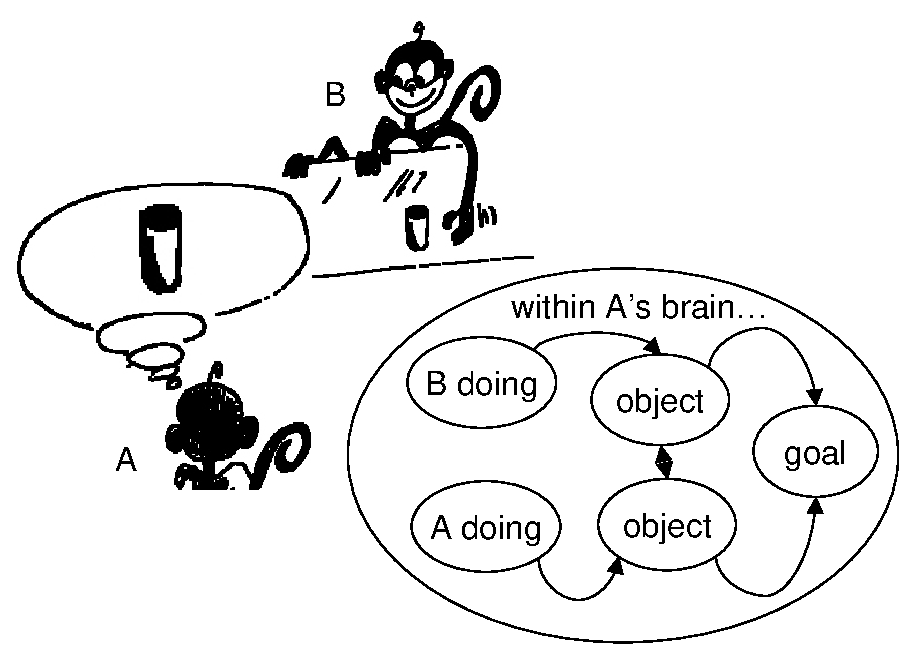
\includegraphics[width=\columnwidth]{mirror-monkey.eps}
\caption{ 
\label{fig:mirror-monkey}
%
Mirror neurons and causality: from the observer's point
of view (A), understanding B's action means mapping it onto the
observer's own
motor repertoire. If the causal chain leading to the goal is already
in place (lower branch of the graph) then the acquisition of a
mirror neuron for this particular action/object is a matter of
building and linking the upper part of the chain to the lower one.
There are various opportunities to reinforce this link either at the object
level, at the goal level or both. 
%%Developmentally we can explain
%%mirror neurons only if we take into account another class of neurons
%%(called canonical) which in practice describes the lower branch of the
%%graph.
%
}
\end{center}
\end{figure}


An interesting question then is
whether the system could extract useful information from seeing an
object manipulated by someone else.  In the case of poking, the robot
needs to be able to estimate the moment of contact and to track the arm
sufficiently well to distinguish it from the object being poked.  We
are interested in how the robot might learn to do this.  One approach
is to chain outwards from an object the robot has poked.  If someone
else moves the object, we can reverse the logic used in poking --
where the motion of the manipulator identified the object -- and
identify a foreign manipulator through its effect on the object.
Poking is an ideal testbed for future work on this, since it is much
simpler than full-blown object manipulation and would only require a
very simple model of the foreign manipulator to work.

There is considerable precedent in the literature for a strong
connection between viewing object manipulation performed by either
oneself or another \cite{wohlsclager02human}.  As we already mentioned
F5 contains a class of neurons called canonical neurons that have a
very specific response when an object is being either manipulated or
fixated.  Grossly simplifying, we might think of canonical neurons as
an association table of grasp/manipulation (action) types with object
(vision) types.  Another class of neurons called ``mirror neurons''
can then be thought of as a second-level association map which links
together the observation of a manipulative action performed by
somebody else with the neural representation of one's own action.

Figure~\ref{fig:mirror-monkey} shows this causal chain in action.
There are a series of interesting behaviors that can be realized based
on mirror neurons. Mimicry is an obvious application, since it
requires just this type of mapping between other and self in terms of
motor actions.  Another important application is the prediction of
future behavior from current actions, or even inverting the causal
relation to find the action that most likely will get to the desired
consequence.

\ifverbose

for example, by observing the part of an action the robot or the
bioagent can come out with suitable expectations of the consequences
of that action. On the other hand, the inverse behavior can also be
foreseen. The latter account to inverting the causal relation and
getting the action that most likely will get to the desired
consequence.

It might be argued that we need a two stages procedure to learn a
mirror representation, where we first learn ``something'' and only
subsequently we ``understand'' other people's behavior. The actual
developmental course might not be such artificially staged. A slight
advantage must be given though to the initial step of self-learning,
the undestanding comes later.


This set of associations can be learnt autonomously (by a robot for
example) simply by a trial and error procedure and possibly with a
reinforcing signal to tell when a given grasp/manipulatory gesture was
successful if applied to a particular object.

We should not probably think of this association as describing in
detail the object being manipulated visually. Perhaps only features
relevant to manipulation are stored (e.g. size, orientation in space).
This representation is a ``pragmatic'' one describing only those
properties of objects are needed to apply a particular set of actions
to them. Affordances are a good psychological analogue of F5
canonical neurons.
\fi


\ifverbose
How does this relate to causation?  The two situations in some sense
share the same goal, and more practically share the same object.  The
whole procedure assumes a basic discrimination of size and shape of
objects (not necessarily categorization in traditional sense), and the
exploitation of the visual information to the understanding of the
grasp type. In some cases though the goal might be unambiguous, e.g. a
needle is very unlikely grasped with a full palm grasp, as well as a
box is not grasped with a pinch grip. These are the most informative
allowing for the best discrimination of action type from the visual
perspective.
\fi

\ifverbose
The definition of imitation we gave here implicitly focus on imitating
the goal rather than the precise trajectory. This automatically takes
into account any difference in body structure between the actor and
the observer.

Of course, manipulation as in poking can lead to a better
understanding of the physical properties of objects not directly
amenable to visual exploration such as mass, roughness, softness, etc.
\fi

\begin{figure}[tbh]
\begin{center}
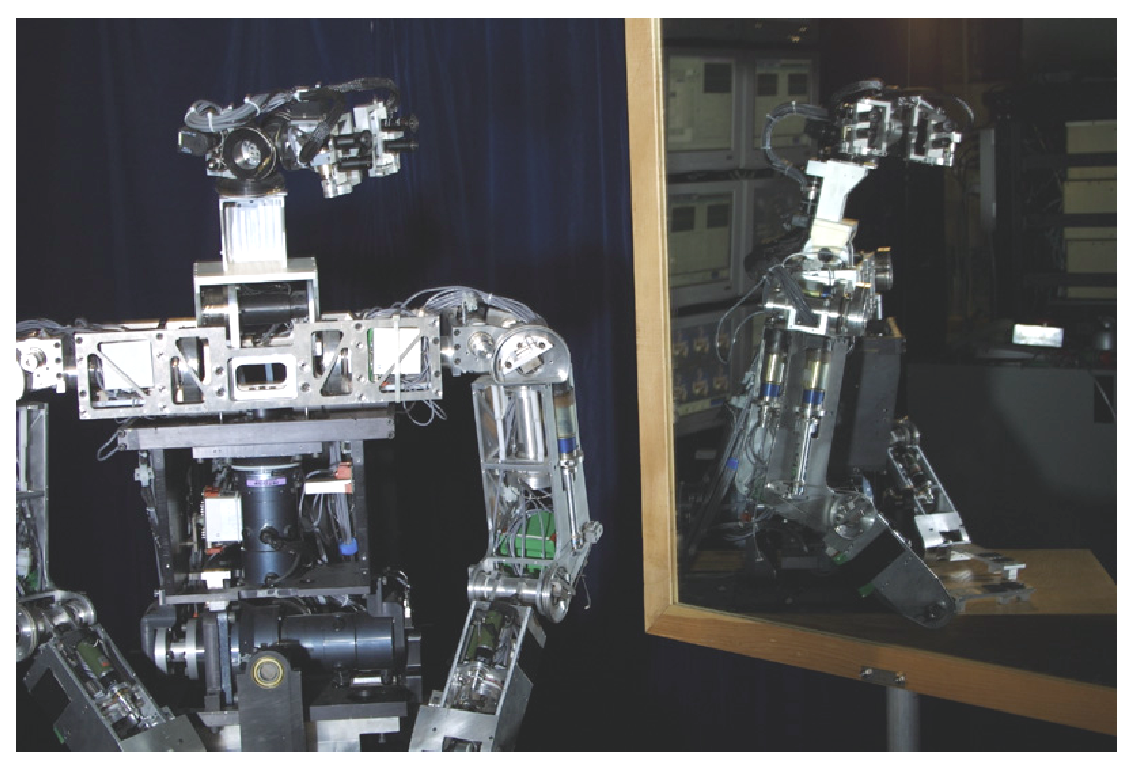
\includegraphics[width=\columnwidth]{mirror-cog.eps}
\caption{ 
\label{fig:mirror-cog}
%
The ultimate goal of this work is for our robot to follow chains of
causation outwards from its own simple body into the complex world.
%
}
\end{center}
\end{figure}


